\documentclass{beamer}
\usepackage{tabularx}
\usepackage{amsmath}
\usepackage{amssymb}
\usepackage{siunitx}
%\usepackage{gensymb}
%\usepackage{graphicx}
%\usepackage{smartdiagram}
\mode<presentation>
{
  %\usetheme{Warsaw}
  % or ...
  \usecolortheme{beaver}

  \setbeamercovered{transparent}
  % or whatever (possibly just delete it)
}
\setbeamertemplate{caption}{\raggedright\insertcaption\par}
\title{Implementation of ADPLL Networks on FPGAs}
\author{Conor Dooley - 14321611}%\\ \newline \and Supervisors: B. Mulkeen \& Dr. E. Blokhina}
\subtitle{Final Presentation}
\date{3 May 2018}
\institute{Supervisors: B. Mulkeen \& Dr. E. Blokhina}

\begin{document}

\begin{frame}
    \titlepage
\end{frame}

\section*{Background/Literature Review}
\begin{frame}{Motivation}
  % - A title should summarize the slide in an understandable fashion
  %   for anyone how does not follow everything on the slide itself.
    \begin{itemize}
        \item[--]
        	Want low power, high frequency clocking system for SoCs.
        \item[--]
            Want closely sync'ed clocks, characterised using:
    		\begin{itemize}
    			\item[]
    				Average difference \textit{skew}.
    			\item[]
	    			Gaussian random process \textit{jitter}.
    		\end{itemize}
    	\item[--]
    		Existing solutions limited by power usage at high frequency.
    	\item[--]
    		ADPLL networks can potentially solve this.
    	\item[--]
    		FPGAs can be used to provide a testbed for ADPLL networks.
    	\item[--]
    		\textbf{Goals}:
    		\begin{itemize}
    			\item[]
    			 Produce such a test platform.
    			\item[]
    				Investigate its performance.
    		\end{itemize}
    	
    \end{itemize}
\end{frame}

\begin{frame}{Existing Solutions}
  % - A title should summarize the slide in an understandable fashion
  %   for anyone how does not follow everything on the slide itself.
	\begin{columns}
		\column{0.55\linewidth}
		\textbf{Branch, H, X trees}
		\begin{itemize}
			\item[--]
				Use buffers \& delay symmetry.
			\item[--]
				Fabrication mismatch problems $\rightarrow$ skew, high power usage.
		\end{itemize}
		\textbf{Clock Mesh}
		\begin{itemize}
			\item[--]
				Great timing accuracy.
			\item[--]
				Redundancy $\rightarrow$ very high power draw.
		\end{itemize}
		\textbf{Skew Compensation}
        \begin{itemize}
        	\item[--]
        		Centralised/Decentralised methods.
	        \item[--]
	            Increases power consumption.
	    \end{itemize}
		\column{0.45\linewidth}
			%\centering	
			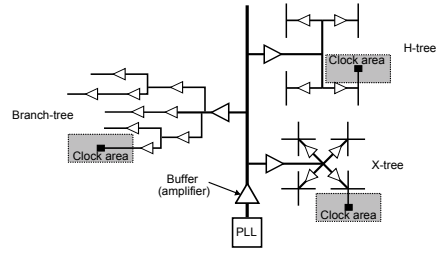
\includegraphics[scale=0.4]{eldar_trees}
			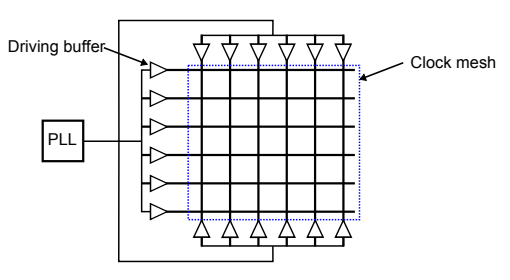
\includegraphics[scale=0.4]{eldar_mesh}
            \begin{flushright}[Zianbetov, 2013]\end{flushright}
	\end{columns}
 
\end{frame}

\begin{frame}{ADPLL Network}
        
        \begin{columns}        	
        	\column{0.6\linewidth}
        	\textbf{ADPLL network:}
	        \begin{itemize}
			    \item[]
			       	ADPLLs generate clock in an area of chip.
			    \item[]
			        Synced via lower freq. error signal between neighbouring PLLs.
       			\item[]
			        Reduces complexity of synchronisation system.
    		\end{itemize}
        	\column{0.4\linewidth}
        	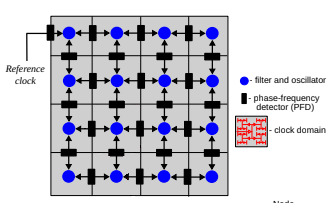
\includegraphics[scale=0.55]{network_ccic2013}
        \begin{flushright}[Zianbetov, 2013]\end{flushright}
        \end{columns}
        \begin{columns}
            \column{\linewidth}
            \vspace{0.1 cm}
    	    \textbf{Example node:}
    	    \begin{center}
		    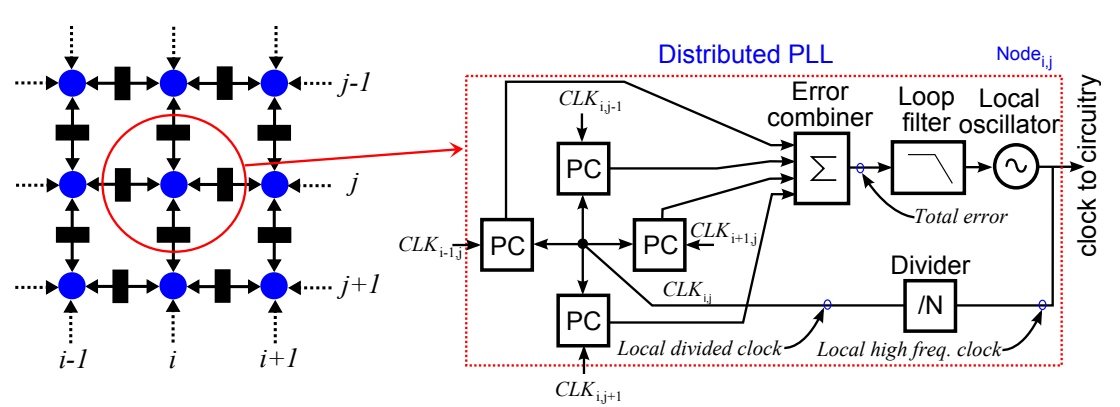
\includegraphics[scale=0.3]{eldar_node}
		    \end{center}
		    %\begin{tiny}\begin{flushright}\cite{eldar}\end{flushright}\end{tiny}
        \end{columns}
\end{frame}

\begin{frame}{Why FPGAs?}

    \begin{itemize}
		\item[--]
			Common verification stage for conventional ASIC designs.
			\begin{itemize}
				\item[]
				Hardware validation of digital circuitry.
				\item[]
				Detection of any potential flaws/errors.
			\end{itemize}
		\item[--]
			Zianbetov \& Shan - Used FPGA to validate ADPLL network:
		\begin{itemize}
			\item[]
				Unable to replicate mixed-signal blocks.
			\item[]
				Operating frequency much lower.
		\end{itemize}
		\item[--]
			Lose precise control over layout.
		\item[--]
			Restriction placed on available hardware.
			\begin{itemize}
				\item[]
					No gates, only LUTs \& primitives.
			\end{itemize} 
		\item[--]
			Limited mixed-signal circuits \textit{are} possible.
		\item[--]
			Can examine system performance and dynamics.
		\item[--]
			Rapid prototyping, minimal cost.	
	
	\end{itemize}
\end{frame}

\begin{frame}{My ADPLL Implementations}
  % - A title should summarize the slide in an understandable fashion
  %   for anyone how does not follow everything on the slide itself.
 	%\begin{columns}
 	\begin{center}
 		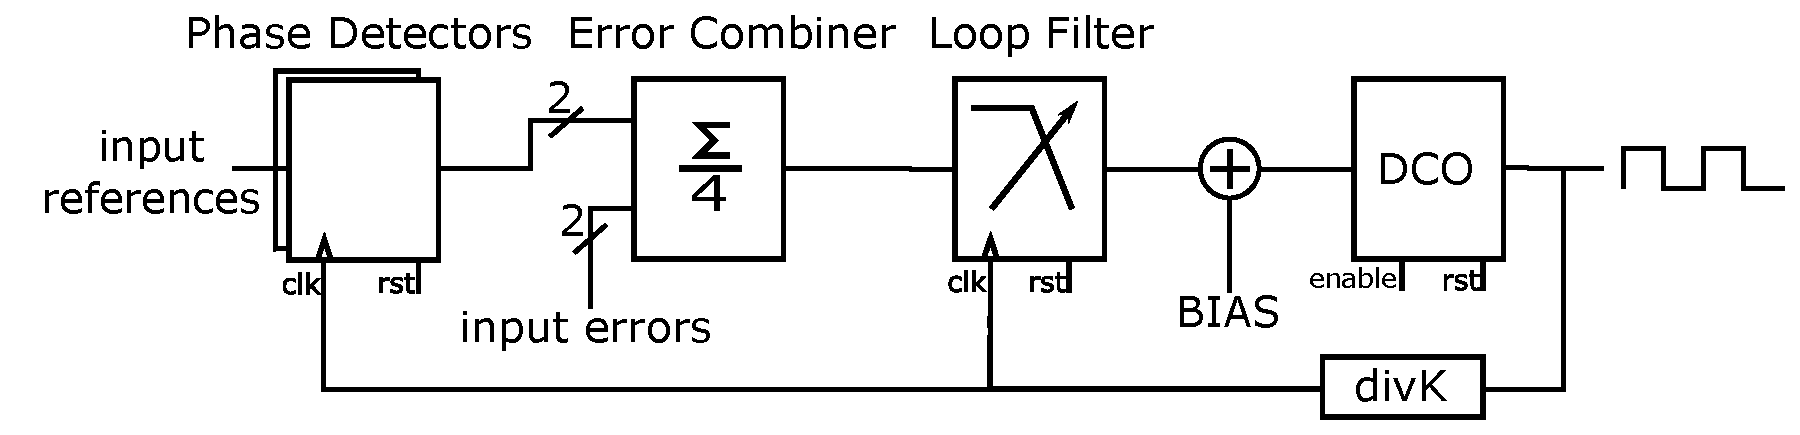
\includegraphics[scale=0.3]{../network_adpll}
 		\vspace{-0.67 cm}
 	\end{center}		
	\begin{itemize}
		\item[--]
			3 different ADPLL designs examined.
		\item[--]
			$5~\si{\mega\hertz}$ centre frequency.
		\item[--]
			Range from entirely FPGA clock driven to entirely inverter delay based.
		\item[--]
			Number of blocks stay the same between designs:
			\begin{itemize}
				\item[]
					Error Combiner,
					Loop Filter,
					Divider.
			\end{itemize}
		\begin{columns}
			\column{0.45\linewidth}
			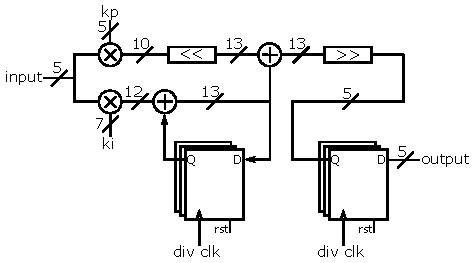
\includegraphics[width=1\linewidth]{../integer_lf}
			\column{0.45\linewidth}
			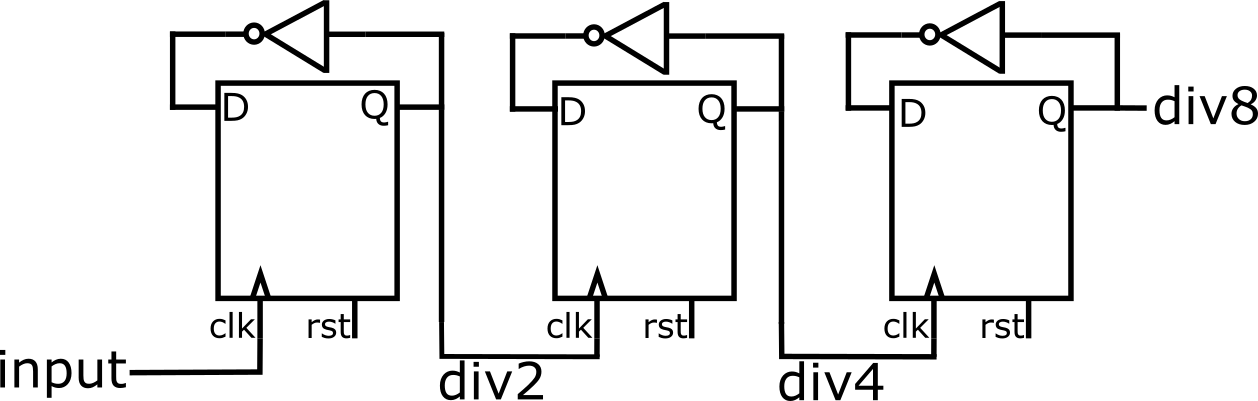
\includegraphics[width=1\linewidth]{../divider2}
		\end{columns}			
	\end{itemize}
	%\end{columns}
\end{frame}

\begin{frame}{Design 1}
% - A title should summarize the slide in an understandable fashion
%   for anyone how does not follow everything on the slide itself.
\vspace{-0.67 cm}

\begin{columns}
	\column{0.45\linewidth}
	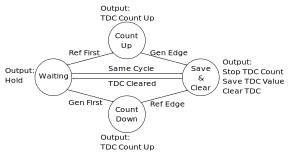
\includegraphics[width=1\linewidth]{../state_trans_new}
	\column{0.45\linewidth}
	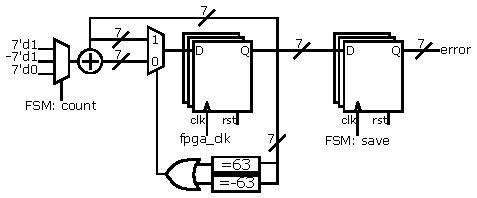
\includegraphics[width=1\linewidth]{../updown}
\end{columns}
\begin{columns}
	\column{0.55\linewidth}
	\begin{itemize}
		\item[--]
		FPGA clocked oscillator and phase detector.
		\item[--]
		Oscillator implemented by accumulator.
		\item[--]
		Phase detector implemented by a statemachine controlling an up-down counter.
		\item[--]
		Worst detector/period resolution of the three designs.
	\end{itemize}
	\column{0.45\linewidth}
	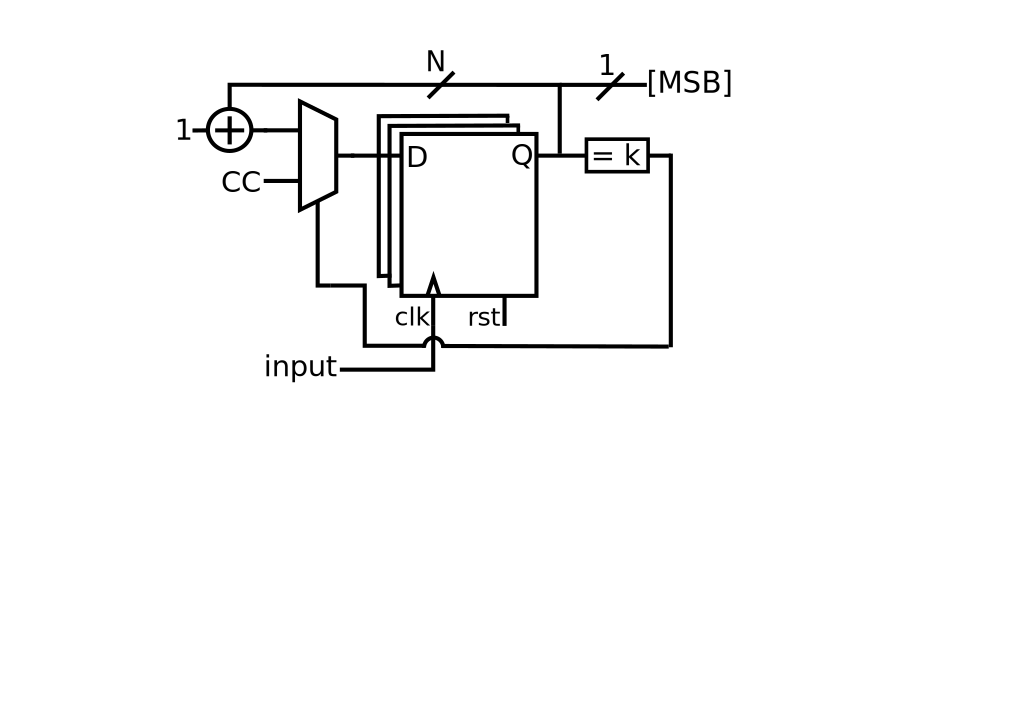
\includegraphics[width=1\linewidth]{../osc1}
\end{columns}

%\end{columns}
\end{frame}

\begin{frame}{Design 2}
% - A title should summarize the slide in an understandable fashion
%   for anyone how does not follow everything on the slide itself.
	\vspace{-0.67 cm}	
	\begin{center}
		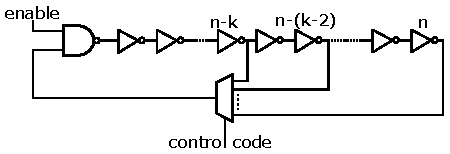
\includegraphics[width=0.8\linewidth]{../ro_new}
	\end{center}
	\vspace{-0.37 cm}
	\begin{columns}
		\column{0.55\linewidth}
		\begin{itemize}
			\item[--]
				Retains FPGA clocked Phase Detector
			\item[--]
				Oscillator replaced by inverter chain using primitives.
			\item[--]
				Better approximation of mixed-signal circuits.
			\item[--]
				Drawback = loss of control.
			\item[--]
				Significant improvement in period resolution, $3.875~\si{\nano\second}\rightarrow \approx 1.1765~\si{\nano\second}$.
		\end{itemize}
		\column{0.45\linewidth}
		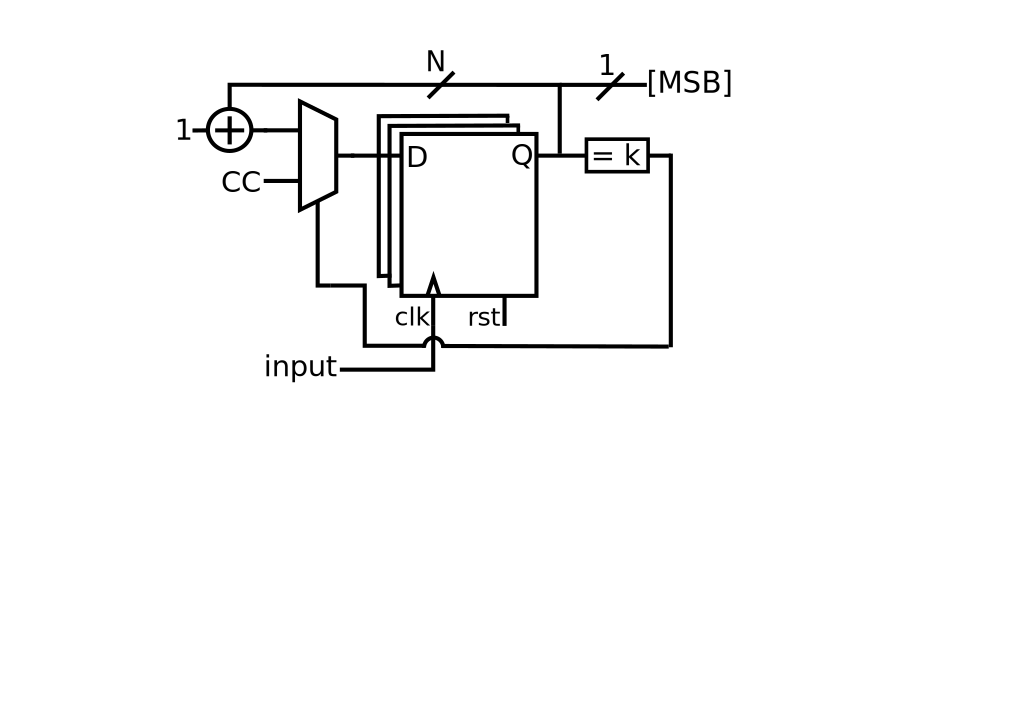
\includegraphics[width=\linewidth]{../osc1}
	\end{columns}
\end{frame}

\begin{frame}{Design 3}
% - A title should summarize the slide in an understandable fashion
%   for anyone how does not follow everything on the slide itself.
	\vspace{-0.4 cm}	
	\begin{center}
		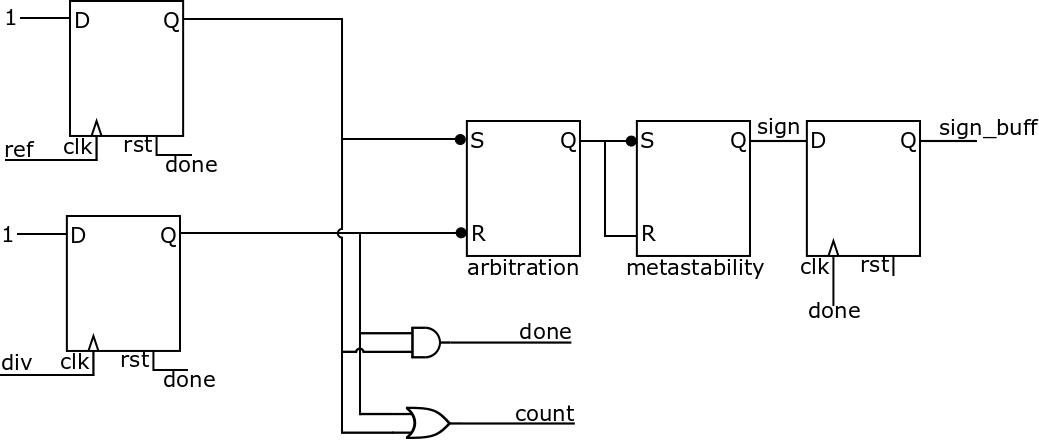
\includegraphics[width=0.75\linewidth]{../new_pdet1}
	\end{center}
	\vspace{-0.4 cm}
	\begin{itemize}
		\item[--]
			Entirely inverter based, retains RO from ADPLL2.
		\item[--]
			SigNum phase detector using inverter primitive TDL.
		\item[--]
			Better approximation of mixed-signal circuits.
		\item[--]
			Loss of control affects range, not centre freq.
		\item[--]
			Detector resolution: $3.875~\si{\nano\second}\rightarrow \approx 0.5883~\si{\nano\second}$.
	\end{itemize}	
	\begin{center}
		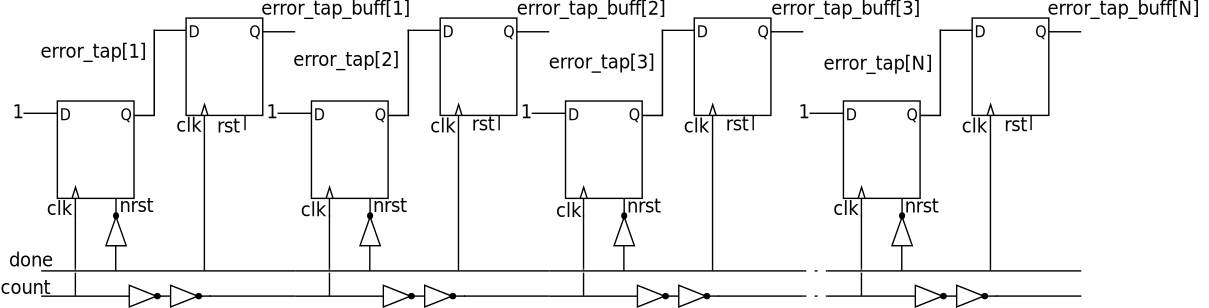
\includegraphics[width=0.75\linewidth]{../new_pdet2}
	\end{center}
\end{frame}

\begin{frame}{ADPLL/Network Performance}
% - A title should summarize the slide in an understandable fashion
%   for anyone how does not follow everything on the slide itself.
	\begin{columns}
		\column{0.45\linewidth}
		\begin{itemize}
			\item[--]
				2x2 \& 3x3 implemented with all designs.
			\item[--]
				Indep. PLL, uni- \& bi-direction mode.
			\item[--]
				Compared all three designs in each mode.
		\end{itemize}
		\column{0.45\linewidth}
		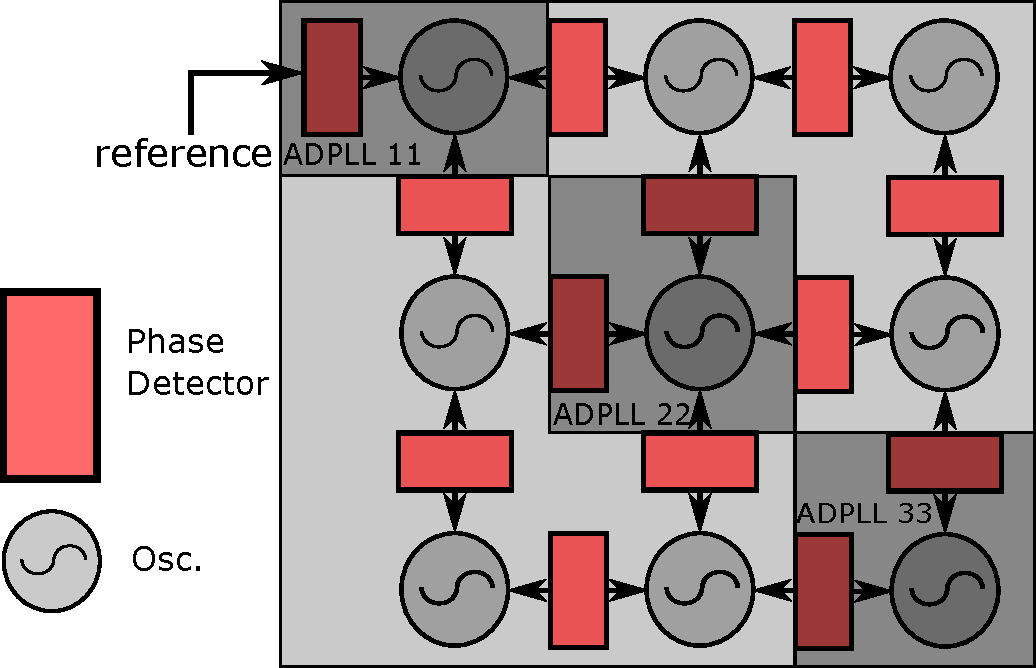
\includegraphics[width=\linewidth]{../network_annotated}
	\end{columns}
	\begin{itemize}
		\item[--]
			Main comparators: Time Interval Error, C2C jitter \& skew.
		\item[--]
			ADPLL 3 top performer overall, but greater C2C jitter.
			\begin{itemize}
				\item[-]
					C2C jitter $\rightarrowtail$ D1: $1.95~\si{\nano\second}$, D2: $0.65~\si{\nano\second}$, D3: $0.75~\si{\nano\second}$
				\item[-]
					Peak TIE $\rightarrowtail$ D1: $19.7~\si{\nano\second}$, D2: $19.1~\si{\nano\second}$, D3: $9.77~\si{\nano\second}$
			\end{itemize} 
		\item[--]
			ADPLL 2 has less C2C jitter as PDet has no variability.
		\item[--]
			ADPLL design 1 suffers most from significant skew issues.
			\begin{itemize}
				\item[]
					Propagation delay due to resolution?
			\end{itemize}  
	\end{itemize}
\end{frame}

\begin{frame}{ADPLL/Network Performance}
% - A title should summarize the slide in an understandable fashion
%   for anyone how does not follow everything on the slide itself.
	\vspace{-0.4 cm}
	\begin{columns}
		\column{0.45\linewidth}
		\begin{figure}
			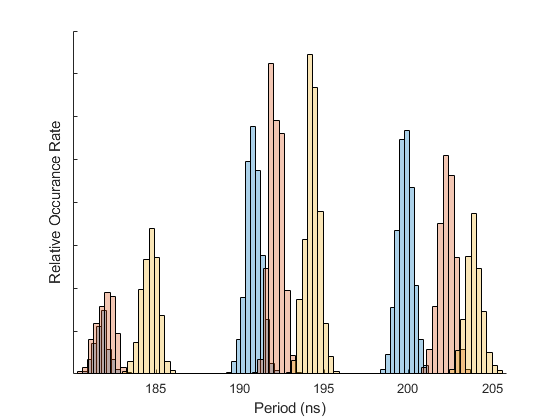
\includegraphics[width=\linewidth]{../conf_paper/distrib_ring}
			\vspace{-0.8 cm}
			\caption{Ring Oscillator}
		\end{figure}
		\column{0.45\linewidth}
		\begin{figure}
			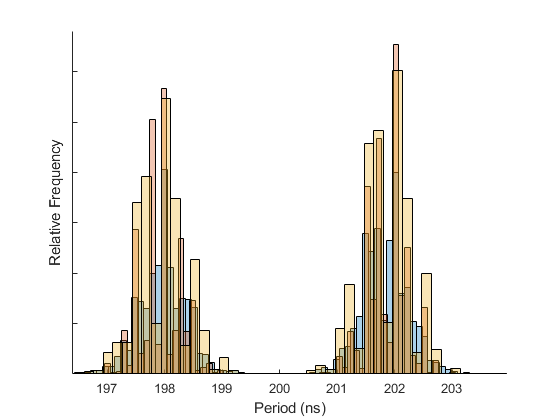
\includegraphics[width=\linewidth]{../conf_paper/distrib_pa}
			\vspace{-0.8 cm}
			\caption{FPGA Clocked Oscillator}
		\end{figure}
	\end{columns}

	\begin{itemize}
		\item[--]
			Period distribution highlights variability missing in clocked oscillator and phase detector designs.
		\item[--]
			Variability of inverter based designs $\rightarrow$ ideal for behavioural investigations.
			\begin{itemize}
				\item[]
					Pierre \& Eugene.
			\end{itemize} 
		\item[--]
			FPGA clocked $\rightarrow$ greaater control, better for design validation.
			\begin{itemize}
				\item[]
					Zianbetov \& Shan.
			\end{itemize} 
			
	\end{itemize}
\end{frame}

\begin{frame}{Minor Variations}
% - A title should summarize the slide in an understandable fashion
%   for anyone how does not follow everything on the slide itself.
\vspace{-0.6 cm}
	\begin{columns}
		\column{0.45\linewidth}
		\begin{itemize}
			\item[--]
			Investigated a number of minor variations in the design.
			\item[--]
			Some to justify decisions:%
			\begin{itemize}
				\item[-]
					Lack of loop filter input delay.
				\item[-]
					Accumulator Width.
			\end{itemize}  
			\item[--]
			Also to test for expected results:
			\begin{itemize}
				\item[-]
					DCO Width Variation
				\item[-]
					LF Comparison with Eugene's results.
				\item[-]
					Impact of feedback divider.
			\end{itemize}
		\end{itemize}
		\column{0.45\linewidth}
		\begin{figure}
			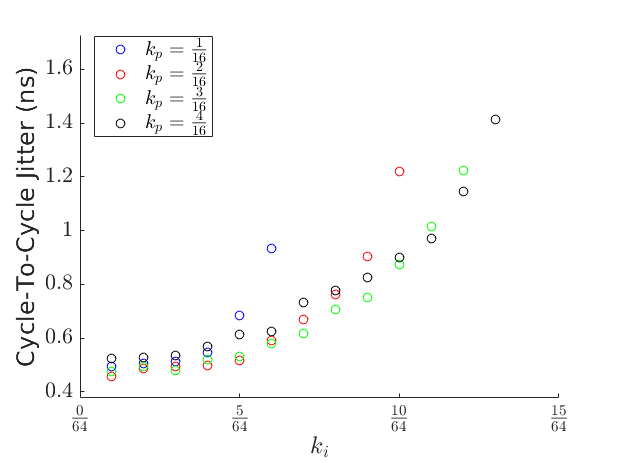
\includegraphics[width=\linewidth]{../fixed_kp_zoom}
			\vspace{-0.8 cm}
			\caption{LF Gain Variation}
		\end{figure}
		\vspace{-1.1 cm}
		\begin{figure}
			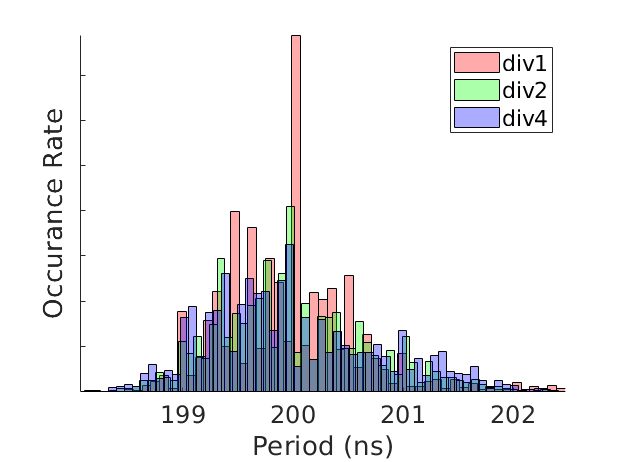
\includegraphics[width=\linewidth]{../dist_2}
			\vspace{-0.8 cm}
			\caption{Impact of Divider}
		\end{figure}
	\end{columns}	
\end{frame}

\iffalse
\begin{frame}{References}
  %\frametitle<presentation>{For Further Reading}
	\begin{columns}
		\column{0.6\linewidth}
		\begin{thebibliography}{10}
		\begin{tiny}
		\setbeamertemplate{bibliography item}{}
		% Followed by interesting articles. Keep the list short.
		\bibitem{read_first}
		M. Javidan, et al.
		\newblock All-digital PLL array provides reliable distributed clock for SOCs.
		\newblock {\em IEEE International Symposium on Circuits and Systems}, 2589-2592, 2011. %PID coefficients	
  	
	  	% Start with overview books.
	  	\bibitem{eldar}
	    E. Zianbetov.
	    \newblock {\em Distributed Clocking For Synchronous SoC}.
		\newblock Universit\'e Pierre et Marie Curie, 2013. %network architecture
		
		\bibitem{shan}
		C. Shan.
		\newblock {\em Distributed Clocking For Synchronous SoC}.
		\newblock Universit\'e Pierre et Marie Curie, 2014. %network architecture
		
	 	 % Followed by interesting articles. Keep the list short.
	  	\bibitem{pid_coeffs}
	    E. Koskin, et al.
	    \newblock Generation of a Clocking Signal in Synchronized All-Digital PLL Networks.
	    \newblock {\em IEEE Transactions on Circuits and Systems II: Express Briefs}, 65(6), 809-813, 2018. %PID coefficients

        \bibitem{_1995}
        G.A. Pratt, and J. Nyugen.
	    \newblock Distributed synchronous clocking.
        \newblock {\em IEEE Transactions on Parallel and Distributed Systems}, 6(3), 314-328, 1995. %PID coefficients

	    
	    \bibitem{sitime}
	    SiTime.
	    \newblock {\em AN10007 Jitter Definitions and Measurement v1.2}.
	    
	    \end{tiny}
        \bibliographystyle{apalike}
	  	\end{thebibliography}
  		\column{0.4\linewidth}
  		\begin{itemize}
  			\vspace{5mm}
  			\item[$\rightarrow$] Background Info
                \vspace{0.8 cm}
  			\item[$\rightarrow$] ADPLL/DCO Design
  			\vspace{0.6 cm}
  			\item[$\rightarrow$] ADPLL Network
  			\vspace{0.6 cm}
  			\item[$\rightarrow$] Filter Coefficients
            \vspace{0.6 cm}
            \item[$\rightarrow$] Initial Proposition
            \item[] ~
  			\item[] ~
            \item[] ~
  		\end{itemize}
  \end{columns}
\end{frame}
\fi

\section*{Summary}

\begin{frame}{Summary}

  % Keep the summary *very short*.
    \begin{itemize}
        \item[--]
            FPGA based analysis platform for ADPLL network designs.
        \item[--]
            Implemented a three ADPLL designs.
        \item[--]
            Compared the designs and impact of minor changes.
        \item[--]
            Implemented 2x2 and 3x3 ADPLL networks using each of the three designs.
        \item[--]
            Proposed suitable use cases for each design.
        \item[--]
        \begin{itemize}
            \textbf{Future Work}:
            \item[-]
            	Larger network.
            \item[-]
            	TDL characterisation.
            \item[-]
            	New FPGA clocked DCO (Period Linear).
           	\item[-]
            	Procedural network instantiation.
        \end{itemize}
    \end{itemize}

\end{frame}

\end{document}
